\documentclass[10pt]{article}

\usepackage[T1]{fontenc}
\usepackage{geometry}
\usepackage{amsmath, amssymb, amsthm}
\usepackage{graphicx}
\usepackage{hyperref}

\title{Geodynamics - Assignment II}
\author{Satvik Saha}
\date{}

\geometry{a4paper, margin=1in}
% \setlength\parindent{0pt}
\renewcommand{\labelenumi}{(\alph{enumi})}

\begin{document}
        \noindent\textbf{IISER Kolkata} \hfill \textbf{Assignment II}
        \vspace{3pt}
        \hrule
        \vspace{3pt}
        \begin{center}
                \LARGE{\textbf{ES 2102 : Hydrology and Geodynamics}}
        \end{center}
        \vspace{3pt}
        \hrule
        \vspace{3pt}
        Satvik Saha, \texttt{19MS154}\hfill\today
        \vspace{20pt}

        We have obtained data on the Bouguer gravity anomaly values in the Himalayas, along a vertical south to north profile through Kathmandu 
        \cite{gravity}. The general trend has been reproduced in the following sketch.
        \begin{center}
                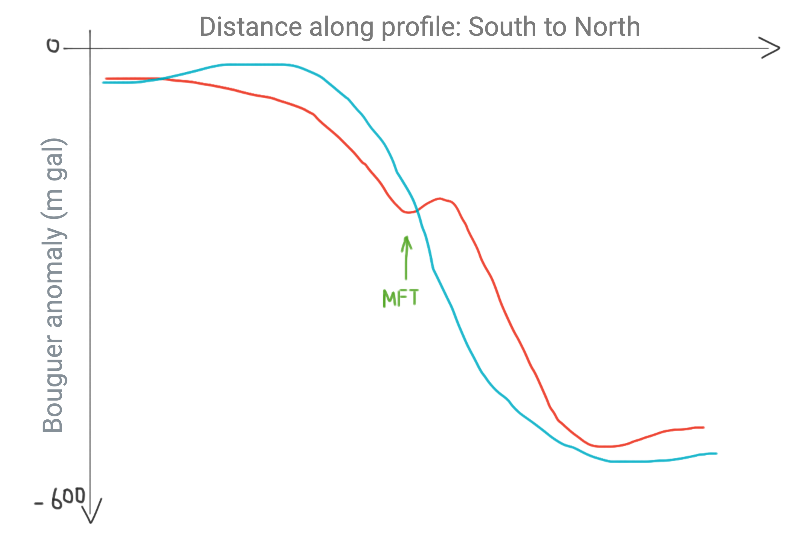
\includegraphics[width=0.6\textwidth]{anomaly.png}
        \end{center}
        The blue line marks the expected anomaly from local Airy isostasy calculations. The red line marks the observed Bouguer anomaly values.
        The green arrow marks the Main Frontal Thrust fault (MFT).

        Note that the crustal thickness in the Gangetic foreland is around 35-40 km, and the crustal thickness beneath Tibet is around
        70-75 km, as estimated from seismic measurements. Using the Bouguer anomaly difference of 460 mgal between the two regions, 
        the density contrast between the crust and upper mantle is estimated as 370 kg/m$^3$.
        Using this data, the blue curve has been constructed; the observed red anomaly is higher than expected in the Gangetic foreland,
        and lower than expected in Tibet (in terms of magnitude). This means that the foreland is overcompensated and the Tibet
        region is undercompensated.
        
        This discrepancy suggests that the Himalayas are supported by lithospheric flexure.
        Essentially, the elastic lithospheric plate supports the weight of the Himalayas and the Tibetan plateau by bending down, which in turn
        flexes the Gangetic plain upwards.
        Thus, the principle of Airy isostasy does not really apply, since tensional and elastic forces must also be taken into account.
        In contrast, Airy isostasy would have suggested that the thicker crust is supported by the asthenosphere, so only a pressure balance would
        have sufficed.

        Flexure is governed by the differential equation
        \[
                D\frac{d^4w}{dx^4} + (\rho_{a} - \rho_{b})gw = q(x),
        \]
        where $w$ is the height depression due the load $q(x)$, $D$ is the flexural rigidity and $\rho_{a}$ and $\rho_{b}$ are the densities
        of the materials above and below the plate.

        Another factor to be considered while explaining this discrepancy is the effect of heat on the lithospheric mantle and crust,
        which means that their density cannot be uniform vertically.
        This is further complicated by the presence of low-density sediments in the foreland, which introduces additional layers in the isostasy
        calculation.

        \begin{thebibliography}{9}
        \bibitem{gravity}
        R. Cattin, G. Martelet, P. Henry, J. P. Avouac, M. Diament, T. R. Shakya,
        Gravity anomalies, crustal structure and thermo-mechanical support of the Himalaya of Central Nepal,
        \textit{Geophysical Journal International}, Volume 147, Issue 2, November 2001, Pages 381--392,
        \textsc{\small DOI:} \texttt{\href{https://doi.org/10.1046/j.0956-540x.2001.01541.x}{10.1046/j.0956-540x.2001.01541.x}}.
        \end{thebibliography}

\end{document}
